\documentclass[]{article}
\usepackage{url}
\usepackage{cite}
\usepackage{listings}

\usepackage[utf8]{inputenc}
\usepackage[english]{babel}

\usepackage[dvipsnames]{xcolor}

%\usepackage{xcolor} % for setting colors
\usepackage{lmodern}
\usepackage{graphicx}
\usepackage{textcomp}
\usepackage{hyperref}
\usepackage{enumerate}
\usepackage[numbers]{natbib}	

% set the default code style
\lstset{
	frame=tb, % draw a frame at the top and bottom of the code block
	tabsize=4, % tab space width
	showstringspaces=false, % don't mark spaces in strings
	numbers=left, % display line numbers on the left
	commentstyle=\color{green}, % comment color
	keywordstyle=\color{blue}, % keyword color
	stringstyle=\color{red} % string color
}

%opening
\title{VTX token retire mechanism test plan}
\author{
		The Volentix team\\
	\texttt{sylvain@volentixlabs.com}
}


\begin{document}

\maketitle


\section{Preparation}

\textbf{Nodes on jungle test net}
	8 nodes
	\begin{enumerate}
		\paragraph{}
		\item v44444444444 
		\item quaremachina
		\item volentixtst5
		\item vltxtknaudit
		\item x111111111111
		\item x22222222222
		\item  x33333333333
		\item  vtx222222222				
	  \end{enumerate}
 
\textbf{Create accounts}
\begin{enumerate}	
\item create v11111111111, v222222222222, v33333333333, v55555555555 *	\color{green} DONE

\end{enumerate} 
 \textbf{Actions}
  		\begin{enumerate}
		  \item Mint 2 test pools of  100000.00000000 ERC-777 VTX on Ropsten
		  \item Deploy TVTX token contracts on v11111111111 
		  \item Deploy custodian on v22222222222
		  \item set v22222222222 permissions for v11111111111
		  \item Issue token pool v33333333333
		  \item Initialize v22222222222 currentbal * {\color{green} DONE} 
		  \item Clear v22222222222 balances buffer * {\color{green} DONE} 
 		  \item register nodes to v22222222222 * {\color{green} DONE}
	 \end{enumerate}
   \textbf{Docker network}\\
  \begin{enumerate}
  	\item eos wallet	* {\color{green} DONE}
  	\item open ethereum 	*	 {\color{green} DONE}
  	\item oracle	*  {\color{green} DONE}
  \end{enumerate}

\section{Tests}

					\begin{enumerate}
					\item \textbf{Precision test}\\
					All nodes send same amount. 	* {\color{green} DONE}
						\begin{enumerate}
						\item amount upper/lower bounds: concordant balance 	*	 {\color{green} DONE}
						\item amount format  	*	 {\color{green} DONE}
						\end{enumerate}
					\item \textbf{Buffer test}\\
					\begin{enumerate}
						\item Nodes all send different amounts 	*	 {\color{green} DONE}
						\item 2/3 Nodes send same amount 	* {\color{green} DONE}
						\item Flooding/DDos 	*  {	\color{green} DONE}
					\end{enumerate}
						\item \textbf{Registration test}DONE\\ 	*	 {\color{green} DONE}
						\item \textbf{Unregistration test}DONE\\	*	 {\color{green} DONE}
						\item \textbf{EOS bandwidth test}\\
						\item \textbf{Persistency test} 	*	 {\color{green} DONE}
							\begin{enumerate}
								\item uptime\textit{} 2 d. 	*	 {\color{green} DONE}
								\item Message to network less than 8 nodes with pesistency 
								\item Iterate through 16 nodes and shut 8 down
								\item Manage if provider is not available. 	* {\color{green} DONE}
								\item Test values from providers 	*	 {\color{green} DONE}
							\end{enumerate}
						\item \textbf{Out of ressouces test}\\ 	*	 {\color{green} DONE}
						\begin{enumerate}
							\item CPU DONE 	*	 {\color{green} DONE}
							\item Memory 
							\item BW
						\end{enumerate}  
				\end{enumerate}
			\section{Considerations}
				\begin{enumerate}
				\item Should there be a mechanism for the case where there is no more values being fed to the oracle, keeping the eth side from issuing for that pool?
			\end{enumerate}  
			
%\begin{figure}
%centering
%	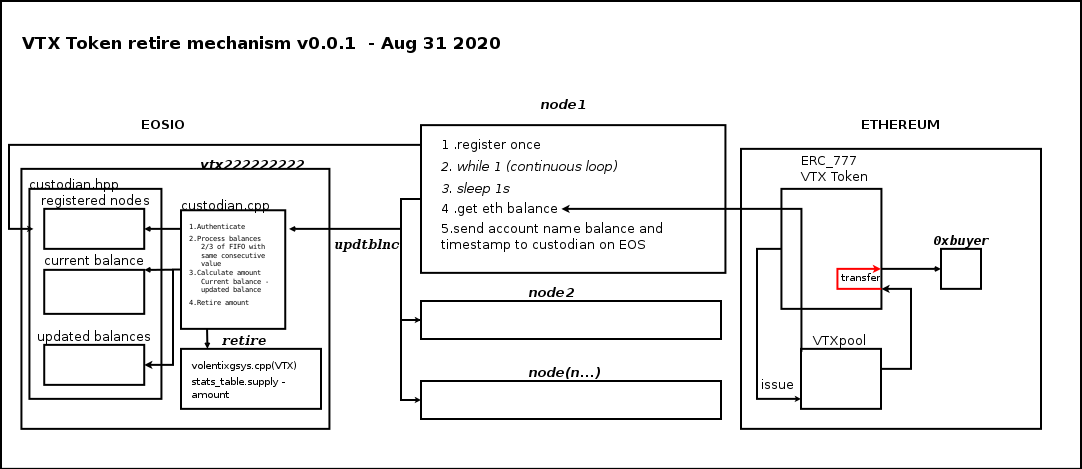
\includegraphics[scale=.33333]{bridge.png}
%\caption{}
%\label{fig:whitebackground-ecosystem02}
%\end{figure}


\end{document}
